\documentclass{article}
\usepackage[utf8]{inputenc}
\usepackage[spanish]{babel}
\usepackage{graphicx}
\graphicspath{ {images/} }
\begin{document}

\begin{titlepage}
    \begin{center}
        \vspace*{1cm}
            
        \Huge
        \textbf{Diseño del proyecto final}
            
        \vspace{0.5cm}
        \LARGE
        Informática II
            
        \vspace{1.5cm}
            
        \textbf{Juan Pablo Areiza Jiménez\\Santiago Montoya Leal}
            
        \vfill
            
        \vspace{0.8cm}
            
        \Large
        Despartamento de Ingeniería Electrónica y Telecomunicaciones\\
        Universidad de Antioquia\\
        Medellín\\
        Octubre de 2021
            
    \end{center}
\end{titlepage}

\tableofcontents
\newpage

\section{Introducción}

Como proyecto final, se busca la realización de un videojuego estilo run and gun, los cuales consisten en personajes que se desplazan a pie, con la posibilidad de ejecutar ataques, saltos y deslizamientos, realizando desplazamientos tanto verticales como horizontales. El videojuego se puede jugar tanto en solitario como en multijugador por turnos, buscando obtener los mejores puntajes y llegar a un alto nivel, así, los jugadores compiten por obtener los mejores resultados. 

\section{Descripción de clases e interacciones}

\begin{itemize}
    \item Personajes: \\Atributos: vidas, posiciones, munición, daño generado por cuchillo y puntaje. \\Métodos: métodos get para obtener los atributos, actualizar posición para todos los tipos de movimiento (salto, deslizamiento, movimiento simple o movimiento armónico), restar vidas, aumentar y restar munción, aumentar puntos o restar puntos en caso de perder nivel.
    \item Enemigos:\\
    Atributos: salud se aumenta en cada nivel, posición. \\Métodos: get y set posición, ataque al comparar la distancia con el personaje 
    \item Bala: \\Atributo: posición, daño generado. \\Métodos: movimiento, get posición y get daño.
    \item Caja: \\Atributos: salud para indicar cuánto se debe golpear hasta destruir, posición y probalidad de item. \\Métodos: set probabilidad (cambia al cambiar de nivel), destruir y generar item (munición, monedas o enemigos adicionales).
    \item Gestión de partidas: \\Atributo: nombre de archivo. \\Métodos: guardar partida, cargar partida, eliminar cuenta y líderes de puntuación
    \item Nivel: \\Atributos: nivel, probabilidad de enemigos, probabilidad de cajas, cantidad de jugadores. \\Métodos: generar enemigo, generar caja, establecer posición de jugador, cambiar de nivel, generar plataforma, generar lianas 
    \item Mainwindow:keypressevent, mover (para generar movimientos aleatorios de enemigos), establecer escena, tiempo por nivel y slots relacionados con botones.
\end{itemize}

\section{Movimientos físicos utilizados}
Movimiento parabólico en salto, deslizamiento de personaje (fricción) y movimiento armónico  usando cuerdas.

\section{Uso de Arduino}
Se utilizará un Arduino leonardo y la librería keyboard para la realización de un control que se pueda utilizar para el videojuego.

\section{Senación de dificultad}
A mayor nivel, más enemigos, además, se cambian las probabilidades de dropeo de las cajas.

\section{Cronograma}
\begin{figure}[h]
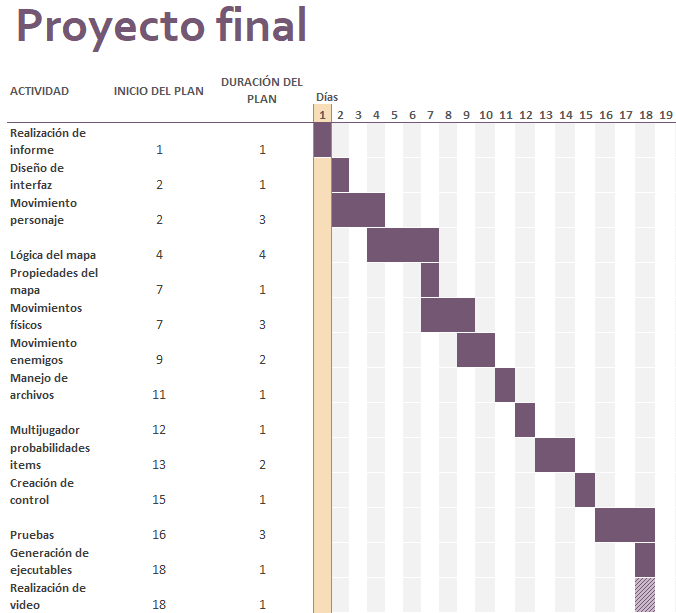
\includegraphics[width=12cm]{Cronograma.PNG}
\centering
\label{fig:Colombia}
\end{figure}

\end{document}
